Modalitatea prin care componentele crawler-ului web "Surf" pot fi accesate, modificate si executate este reprezentata de o interfata\cite{iterface-definition} structurata sub forma unui API RESTful\footnote{engl. \textit{RESTful} = adjectiv de la substantivul \textit{REST}; un API este \textit{RESTful} daca adopta stilul arhitectural \textit{REST\cite{rest-definition}}}. API-ul adopta stilul arhitectural REST\cite{rest-definition} deoarece acesta ajuta la decuplarea arhitecturii si simplificarea urmaririi executiei aplicatiei prin faptul ca nu permite memorarea starilor intermediare in cadrul unei sesiuni de comunicare intre utilizator si crawler. De asemenea, API-ul RESTful confera extensibilitate si flexibilitate la nivel de interfata, intrucat permite gruparea resurselor in mod ierarhic si identificarea usoara a resurselor si a consecintelor aplicarii anumitor actiuni, prin verbe HTTP, asupra starii sistemului. \textit{Figura 8} prezinta secventa mimima de operatii ce trebuie efectuate, la nivel de API, pentru a putea obtine rezultate in urma procesului de parcurgere a paginilor web de catre crawler, modelate printr-o diagrama de secventa.

% Locatie creare diagrama secventa: http://gojs.net/latest/samples/sequenceDiagram.html
% Script creare diagrama secventa:
\iffalse
{ "class": "go.GraphLinksModel",
  "nodeDataArray": [
{"key":"User", "text":"Utilizator", "isGroup":true, "loc":"0 0", "duration":19},
{"key":"Api", "text":"API-ul 'Surf'", "isGroup":true, "loc":"250 0", "duration":19},
{"key":"Backend", "text":"Backend AWS", "isGroup":true, "loc":"500 0", "duration":19},
{"group":"User", "start":1, "duration":4},
{"group":"Api", "start":1, "duration":3},
{"group":"Backend", "start":2, "duration":2},
{"group":"User", "start":6, "duration":4},
{"group":"Api", "start":6, "duration":3},
{"group":"Backend", "start":7, "duration":2},
{"group":"User", "start":11, "duration":4},
{"group":"Api", "start":11, "duration":3},
{"group":"Backend", "start":12, "duration":2},
{"group":"User", "start":16, "duration":4},
{"group":"Api", "start":16, "duration":3},
{"group":"Backend", "start":17, "duration":2}
 ],
  "linkDataArray": [
{"from":"User", "to":"Api", "text":"POST /workflows", "time":1},
{"from":"Api", "to":"Backend", "text":"Validare & inregistrare workflow", "time":2},
{"from":"Backend", "to":"Api", "text":"Workflow din baza de date :id_workflow", "time":3},
{"from":"Api", "to":"User", "text":"Workflow din baza de date :id_workflow", "time":4},
{"from":"User", "to":"Api", "text":"POST /workflows/executions :id_workflow", "time":6},
{"from":"Api", "to":"Backend", "text":"Porneste workflow", "time":7},
{"from":"Backend", "to":"Api", "text":"Executie cu id :id_executie", "time":8},
{"from":"Api", "to":"User", "text":"Executie cu id :id_executie", "time":9},
{"from":"User", "to":"Api", "text":"GET /workflows/executions/:id_executie", "time":11},
{"from":"Api", "to":"Backend", "text":"Listeaza executie", "time":12},
{"from":"Backend", "to":"Api", "text":"Detalii executie", "time":13},
{"from":"Api", "to":"User", "text":"Detalii executie", "time":14},
{"from":"User", "to":"Api", "text":"GET /workflows/executions/:id_executie/metadata", "time":16},
{"from":"Api", "to":"Backend", "text":"Listeaza metadatele asociate executiei :id_executie", "time":17},
{"from":"Backend", "to":"Api", "text":"Metadate asociate cu :id_executie", "time":18},
{"from":"Api", "to":"User", "text":"Metadate asociate cu :id_executie", "time":19}
 ]}
\fi

\begin{figure}[ht]
\begin{center}
	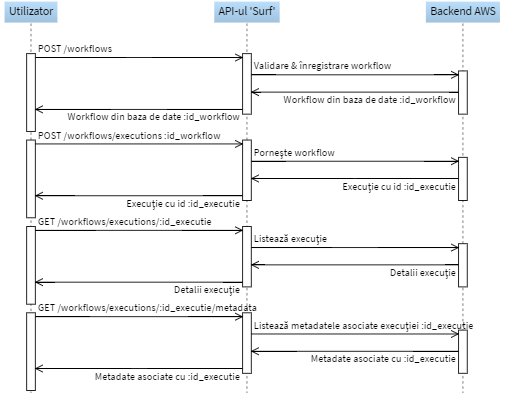
\includegraphics[keepaspectratio, width=0.9\textwidth]{diagrama-utilizator-api.png}
	\caption{Interactiunea utilizator - API \cite{diagram-icons-sources, aws-icons-source}}\par\medskip 

\end{center}
\end{figure}